\documentclass[a4paper,11pt]{article}

\usepackage[T1]{fontenc}
\usepackage[utf8]{inputenc}
\usepackage{graphicx}
\usepackage{xcolor}
\usepackage[fleqn]{amsmath}
\usepackage{tgtermes}
\usepackage[final]{pdfpages}
\usepackage{wrapfig}

\usepackage[normalem]{ulem}
\useunder{\uline}{\ul}{}

\usepackage[
pdftitle={Lingwistyka Formalna i Automaty},
pdfauthor={evemorgen, AGH},
colorlinks=true,linkcolor=blue,urlcolor=blue,citecolor=blue,bookmarks=true,
bookmarksopenlevel=2]{hyperref}
\usepackage{amsmath,amssymb,amsthm,textcomp}
\usepackage{enumerate}
\usepackage{multicol}
\usepackage{tikz}
\usepackage{geometry}
\geometry{
 a4paper,
 total={170mm,257mm},
 left=20mm,
 top=20mm,
}

% custom footers and headers
\usepackage{fancyhdr,lastpage}
\pagestyle{fancy}
\lhead{}
\chead{}
\rhead{}
\lfoot{Assignment \textnumero{} 3}
\cfoot{}
\rfoot{Page \thepage\ /\ \pageref*{LastPage}}
\renewcommand{\headrulewidth}{0pt}
\renewcommand{\footrulewidth}{0pt}
%

%%%----------%%%----------%%%----------%%%----------%%%

\begin{document}

\title{Lingwistyka Formalna i Automaty - ćwiczenia 3}
\author{evemorgen, AGH}
\date{04/12/2016}
\maketitle

\newpage
\section{Dany jest NAS:}
\begin{center}
	\begin{tabular}{rcc}
		\hline
		\multicolumn{1}{|r|}{}     & \multicolumn{1}{l|}{0}      & \multicolumn{1}{l|}{1}         \\ \hline
		\multicolumn{1}{|r|}{> q1} & \multicolumn{1}{l|}{\{q1\}} & \multicolumn{1}{l|}{\{q1,q2\}} \\ \hline
		\multicolumn{1}{|r|}{q2}   & \multicolumn{1}{l|}{\{q3\}} & \multicolumn{1}{l|}{\{q3\}}    \\ \hline
		\multicolumn{1}{|r|}{q3}   & \multicolumn{1}{l|}{\{q4\}} & \multicolumn{1}{l|}{\{q4\}}    \\ \hline
		\multicolumn{1}{|r|}{*q4}  & \multicolumn{1}{l|}{None}   & \multicolumn{1}{l|}{None}      \\ \hline
	\end{tabular}
\end{center}
\subsection{Opisać język opisywany przez NAS}
\begin{center}
	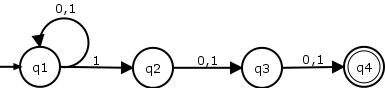
\includegraphics{nas1} \\
	Wszystkie słowa binarne które mają 1 na trzecim miejscu od końca
\end{center}

\subsection{Przekonwertować NAS na DAS}
\begin{center}
	\begin{tabular}{|l|l|l|}
		\hline
		                               & 0                    & 1                        \\ \hline
		>\{q1\} \textbf{A}             & {\ul \{q1\}}         & {\ul \{q1,q2\}}          \\ \hline
		\{q2\}                         & {\ul \{q3\}}         & {\ul \{q3\}}             \\ \hline
		\{q3\}                         & {\ul \{q4\}}         & {\ul \{q4\}}             \\ \hline
		*\{q4\}                        & None                 & None                     \\ \hline
		\{q1, q2\} \textbf{B}          & {\ul \{q1, q3\}}     & {\ul \{q1, q2, q3\}}     \\ \hline
		\{q1, q3\} \textbf{C}          & \{q1, q4\}           & {\ul \{q1, q2, q4\}}     \\ \hline
		*\{q1, q4\} \textbf{E}         & {\ul \{q1\}}         & {\ul \{q1, q2\}}         \\ \hline
		\{q1, q2, q3\} \textbf{D}      & {\ul \{q1, q3, q4\}} & {\ul \{q1, q2, q3, q4\}} \\ \hline
		*\{q1, q2, q4\} \textbf{F}     & {\ul \{q1, q3\}}     & {\ul \{q1, q2, q3\}}     \\ \hline
		*\{q1, q3, q4\} \textbf{G}     & {\ul \{q1, q4\}}     & {\ul \{q1, q2, q4\}}     \\ \hline
		*\{q1, q2, q3, q4\} \textbf{H} & {\ul \{q1, q3, q4\}} & {\ul \{q1, q2, q3, q4\}} \\ \hline
	\end{tabular}
	\hspace{1cm}
	\begin{tabular}{|c|c|}
		\hline
		A & \{q1\}             \\ \hline
		B & \{q1, q2\}         \\ \hline
		C & \{q1, q3\}         \\ \hline
		D & \{q1, q2, q3\}     \\ \hline
		E & \{q1, q4\}         \\ \hline
		F & \{q1, q2, q4\}     \\ \hline
		G & \{q1, q3, q4\}     \\ \hline
		H & \{q1, q2, q3, q4\} \\ \hline
	\end{tabular}
	\\
	\vspace{1cm}

	Czyli ostatecznie \\
	\begin{tabular}{cc}
		\hline
		\raisebox{-\totalheight}{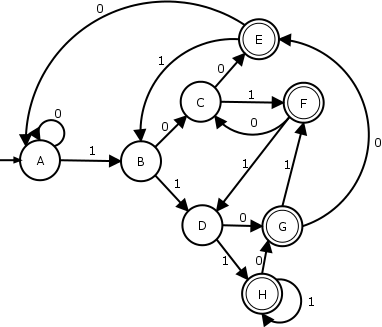
\includegraphics[scale=0.5]{das1}}
		&
		\raisebox{-\totalheight +1.5cm}{
		\begin{tabular}{|c|c|c|}
		   & 0 & 1 \\ \hline
		>A & A & B \\ \hline
		B  & C & D \\ \hline
		C  & E & F \\ \hline
		D  & G & H \\ \hline
		*E & A & B \\ \hline
		*F & C & D \\ \hline
		*G & E & F \\ \hline
		*H & G & H \\ \hline
	\end{tabular}
	}
	\end{tabular}
\end{center}

\newpage
\section{Dany jest NAS:}
\begin{center}
	\begin{tabular}{rcc}
		\hline
		\multicolumn{1}{|r|}{}     & \multicolumn{1}{l|}{0}      & \multicolumn{1}{l|}{1}         \\ \hline
		\multicolumn{1}{|r|}{> q1} & \multicolumn{1}{l|}{\{q1\}} & \multicolumn{1}{l|}{\{q1,q2\}} \\ \hline
		\multicolumn{1}{|r|}{q2}   & \multicolumn{1}{l|}{\{q3\}} & \multicolumn{1}{l|}{None}      \\ \hline
		\multicolumn{1}{|r|}{*q3}  & \multicolumn{1}{l|}{None}   & \multicolumn{1}{l|}{None}      \\ \hline
	\end{tabular}
\end{center}
\subsection{Opisać język opisywany przez NAS}
\begin{center}
	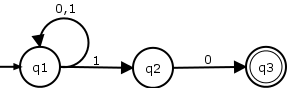
\includegraphics{nas2} \\
	Wszystkie słowa binarne kończące się na 10
\end{center}
\subsection{Przekonwertować NAS na DAS}
\begin{center}
	\begin{tabular}{|l|l|l|}
		\hline
		                       & 0          & 1          \\ \hline
		>\{q1\} \textbf{A}     & \{q1\}     & \{q1, q2\} \\ \hline
		\{q2\}                 & \{q3\}     & None       \\ \hline
		*\{q3\}                & None       & None       \\ \hline
		\{q1, q2\} \textbf{B}  & \{q1, q3\} & \{q1, q2\} \\ \hline
		*\{q1, q3\} \textbf{C} & \{q1\}     & \{q1, q2\} \\ \hline

	\end{tabular}
	\hspace{1cm}
	\begin{tabular}{|l|l|}
		\hline
		A & \{q1\}     \\ \hline
		B & \{q1, q2\} \\ \hline
		C & \{q1, q3\} \\ \hline
	\end{tabular}
	\\
	\vspace{1cm}

	Czyli ostatecznie \\
	\begin{tabular}{cc}
		\hline
		\raisebox{-\totalheight}{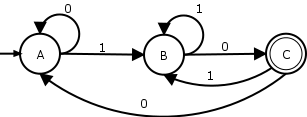
\includegraphics[scale=0.7]{das2}}
		&
		\raisebox{-\totalheight}{
		\begin{tabular}{|c|c|c|}
		\hline
		   & 0 & 1 \\ \hline
		>A & A & B \\ \hline
		B  & C & B \\ \hline
		*C & A & B \\ \hline
	\end{tabular}
	}
	\end{tabular}
\end{center}

\newpage
\section{Dany jest NAS:}
\begin{center}
	\begin{tabular}{rcc}
		\hline
		\multicolumn{1}{|r|}{}     & \multicolumn{1}{l|}{0}         & \multicolumn{1}{l|}{1}         \\ \hline
		\multicolumn{1}{|r|}{> q1} & \multicolumn{1}{l|}{\{q1\}}    & \multicolumn{1}{l|}{\{q1,q2\}} \\ \hline
		\multicolumn{1}{|r|}{q2}   & \multicolumn{1}{l|}{\{q3,q4\}} & \multicolumn{1}{l|}{\{q3\}}    \\ \hline
		\multicolumn{1}{|r|}{q3}   & \multicolumn{1}{l|}{None}      & \multicolumn{1}{l|}{\{q4\}}    \\ \hline
		\multicolumn{1}{|r|}{*q4}  & \multicolumn{1}{l|}{\{q1\}}    & \multicolumn{1}{l|}{\{q2\}}    \\ \hline
	\end{tabular}
\end{center}
\subsection{Przekonwertować NAS na DAS}
\begin{center}
	\begin{tabular}{|l|l|l|}
		\hline
		                               & 0                    & 1                        \\ \hline
		>\{q1\} \textbf{A}             & {\ul \{q1\}}         & {\ul \{q1, q2\}}         \\ \hline
		\{q2\}                         & {\ul \{q3, q4\}}     & {\ul \{q3\}}             \\ \hline
		\{q3\}                         & None                 & {\ul \{q4\}}             \\ \hline
		*\{q4\}                        & {\ul \{q1\}}         & {\ul \{q2\}}             \\ \hline
		\{q1, q2\} \textbf{B}          & {\ul \{q1, q3, q4\}} & {\ul \{q1, q2, q3\}}     \\ \hline
		*\{q3, q4\}                    & {\ul \{q1\}}         & {\ul \{q2, q4\}}         \\ \hline
		*\{q2, q4\}                    & {\ul \{q1, q3, q4\}} & {\ul \{q2, q3\}}         \\ \hline
		\{q2, q3\}                     & {\ul \{q3, q4\}}     & {\ul \{q3, q4\}}         \\ \hline
		\{q1, q2, q3\} \textbf{D}      & {\ul \{q1, q3, q4\}} & {\ul \{q1, q2, q3, q4\}} \\ \hline
		*\{q1, q3, q4\} \textbf{C}     & {\ul \{q1\}}         & {\ul \{q1, q2, q4\}}     \\ \hline
		*\{q1, q2, q4\} \textbf{E}     & {\ul \{q1, q3, q4\}} & {\ul \{q1, q2, q3\}}     \\ \hline
		*\{q1, q2, q3, q4\} \textbf{F} & {\ul \{q1, q3, q4\}} & {\ul \{q1, q2, q3, q4\}} \\ \hline
	\end{tabular}
	\hspace{1cm}
	\begin{tabular}{|l|l|}
		\hline
		A & \{q1\}             \\ \hline
		B & \{q1, q2\}         \\ \hline
		C & \{q1, q3, q4\}     \\ \hline
		D & \{q1, q2, q3\}     \\ \hline
		E & \{q1, q2, q4\}     \\ \hline
		F & \{q1, q2, q3, q4\} \\ \hline
	\end{tabular}
	\\
	\vspace{1cm}
	Czyli ostatecznie
	\\
	\begin{tabular}{cc}
    	\hline
		\raisebox{-\totalheight}{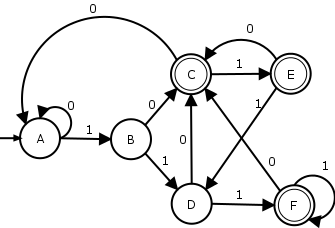
\includegraphics[scale=0.8]{das3}}
		&
		\raisebox{-\totalheight}{
		\begin{tabular}{|c|c|c|}
		\hline
		   & 0 & 1 \\ \hline
		>A & A & B \\ \hline
		B  & C & D \\ \hline
		*C & A & E \\ \hline
		D  & C & F \\ \hline
		*E & C & D \\ \hline
		*F & C & F \\ \hline
	\end{tabular}
	}
	\end{tabular}
\end{center}
\end{document}
